\documentclass{article}
\usepackage[utf8]{inputenc}

\usepackage{tikz}
\usetikzlibrary{positioning}



\title{Kafka Project}
\author{Mislav Jakšić}
\date{\today{}}



\begin{document}

\maketitle

Koristi Java 8

Korist Spring Boot, za REST API

Pretpostavljen je intranet radi sigurnosti

Hamag Bicro agencija, veliki projekt

Napraviti minimalni UI koji se koristi samo za testiranje

Napraviti jednu po jednu "vertikalu" CRUDL (create, read, update, delete, list)

S Zookeeperom uspostavi vezu s zkClient, program na GitHub-u

S Kafkom uspostavi vezu koristeci AdminClient

Koristi verziju Kafka ili 2.1 ili 0.11

Tri moguce arhitekture: mikrousluge, monolit ili server klijent

Nemogu se izvesti sve CRUDL operacija za sve resurse

Resursi Kafka koji su bitni su: topics, partitions, messages, consumers, producers, streams

Kafka API se mijenja cesto: omotaj svaku Kafka funkciju sa svojom vlastitom



\begin{figure}
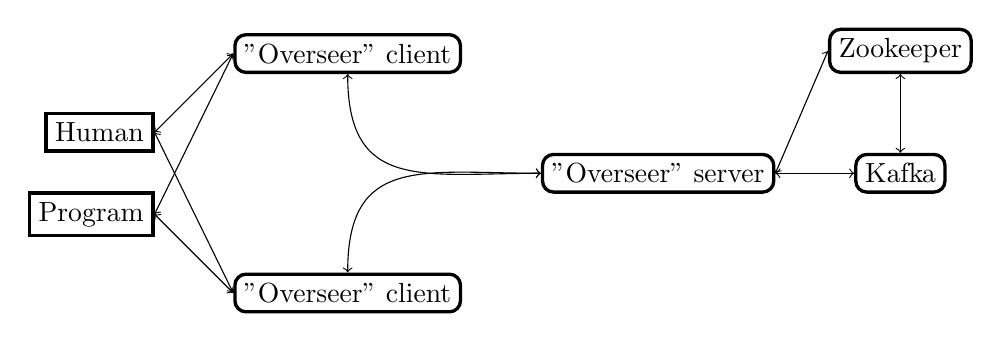
\begin{tikzpicture}[ % has a lot of options; consult the manual
square/.style={rectangle, draw=black, very thick},
square_rounded/.style={rectangle, rounded corners, draw=black, very thick},
]

% \node[type](name_of_node)[above/below/right/left/...=of name_of_node]{text_in_node}
\node[square_rounded](zookeeper_one){Zookeeper};
\node[square_rounded](kafka_one)[below=of zookeeper_one]{Kafka};

\node[square_rounded](server_one)[left=of kafka_one]{"Overseer" server};

\node[square_rounded](client_one)[above left=of server_one]{"Overseer" client};
\node[square_rounded](client_two)[below left=of server_one]{"Overseer" client};

\node[square](human_one)[left=of client_one, yshift=-10mm]{Human};
\node[square](program_one)[left=of client_two, yshift=10mm]{Program};

% \draw[->] (name_of_node.direction) -- (name_of_node.direction)
\draw[<->] (zookeeper_one.south) -- (kafka_one.north);

\draw[<->] (server_one.east) -- (zookeeper_one.west);
\draw[<->] (server_one.east) -- (kafka_one.west);

\draw[<->] (client_one.south) .. controls +(down:15mm) and +(left:15mm) .. (server_one.west);
\draw[<->] (client_two.north) .. controls +(up:15mm) and +(left:15mm) .. (server_one.west);

\draw[<->] (human_one.east) -- (client_one.west);
\draw[<->] (human_one.east) -- (client_two.west);

\draw[<->] (program_one.east) -- (client_one.west);
\draw[<->] (program_one.east) -- (client_two.west);

\end{tikzpicture}
\end{figure}



\end{document}
